\newpage
\section{Design af database} \label{sec:ER}
Det ønskes, at brugerdata er knyttet til den enkelte bruger i databasen. Dette er med henblik på, at app'en ikke skal lagre større mængder data på den mobile enhed samt sikre data i tilfælde af uforudsete hændelser, som eksempelvis tab af mobil enhed. Databasen skal indeholde oplysninger om de enkelte KOL-patienter, herunder resultater opnået ved træning og vennerelation. 

\subsection{ER-diagram}
Modellering af databasen udarbejdes ud fra et ER-diagram. ER-diagrammet relaterer sig til én KOL-patient i databasen. Databasen tager udgangspunkt i entiteter som KOL-patient, vennerelation, konditionstræning og belønninger. Disse entiteter har tilhørende attributter, som ses af ER-diagrammet for databasen i \autoref{fig:ERdiagram}.

\begin{figure} [H]
\centering
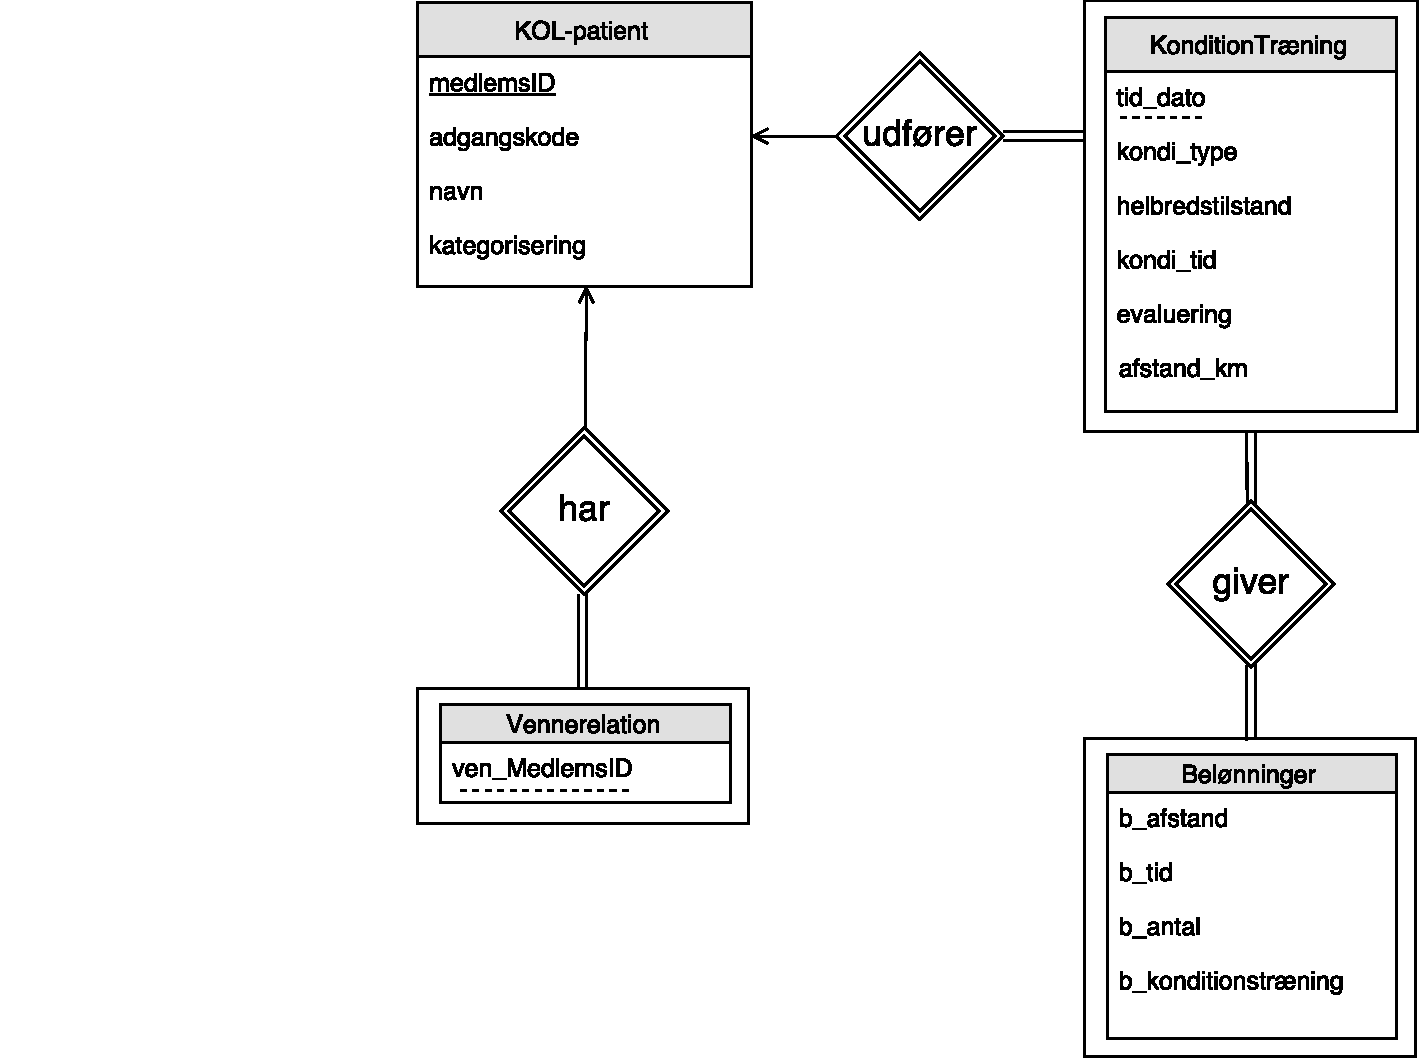
\includegraphics[width=1\textwidth]{figures/Aktivitetsdiagram/ERdiagram}
\caption{ER-diagram for database.}
\label{fig:ERdiagram}
\end{figure} 

\noindent
Af \autoref{fig:ERdiagram} ses ER-diagrammet over databasen, hvori KOL-patienter oprettes og informationer om patienterne samt deres resultater lagres. Den enkelte KOL-patient er en stærk entitiet, som registreres med primærnøglen, \textit{medlemsID}. Derudover fremgår de svage entiteter, herunder \textit{Vennerelation}, \textit{KonditionTræning} og \textit{Belønninger}. Én KOL-patient har mange vennerelationer, som kan identificeres ved KOL-patientens \textit{medlemsID} og \textit{venMedlemsID}. Det samme gør sig gældende for konditionstræninger, hvor én KOL-patient kan udføre mange konditionstræninger, der identificeres ved \textit{tid\_dato} og \textit{medlemsID}. Ligeledes kan belønninger, som er en mange til mange relation, identificeres ved \textit{b\_tid\_dato} og \textit{medlemsID}.

\subsection{Schema}
ER-diagrammet omskrives til schema for at kunne normalisere og implementere databasen. Normaliseringen anvendes med henblik på at reducere redundans og inkonsistens. Schema er i anden normalform og fremgår af \autoref{tab:schema}. 
Første normalform opnås ved at gøre alle attributter anatomiske. Navn, fra entiteten, KOL-patient, opdeles i fornavn og efternavn for at opnå første normalform. For at opnå anden normalform skal første normalform opnås, og alle attributter i en tabel skal være afhængige af en primærnøgle. Ved tredje normalform må det ikke være tilfældet, at en attribut er funktionel afhængig af en anden attribut, som er funktionel afhængig af primærnøglen. Schemaet på trejde normalform ses på \autoref{tab:schema}.

\begin{table} [H]
	\centering
  \begin{tabular}{ | l | p{12cm} |} \hline
     \textbf{Stærke entiteter} & KOL-patient = (\underline{medlemsID}, adgangskode, fornavn, efternavn, kategorisering) \\ \hline
 	\textbf{Svage entiteter} & Træning = (\underline{medlemsID}, \underline{tid$\_$dato}, kondi$\_$type, helbredstilstand, kondi$\_$tid, afstand$\_$km, evaluering)
 \newline Vennerelation = (\underline{medlemsID}, \underline{venMedlemsID})
\newline Belønninger = (\underline{medlemsID}, \underline{b$\_$tid$\_$dato}, b$\_$afstand, b$\_$tid, b$\_$antal, b$\_$konditionstræning)\\ \hline
    \end{tabular}
    \caption{ER-diagram for databasen omskrevet til schema på første, anden og tredje normalform.}
    \label{tab:schema}
\end{table}

